\documentclass[12pt, twoside]{article}
\usepackage[letterpaper, margin=1in, headsep=0.2in]{geometry}
\setlength{\headheight}{0.6in}
%\usepackage[english]{babel}
\usepackage[utf8]{inputenc}
\usepackage{microtype}
\usepackage{amsmath}
\usepackage{amssymb}
%\usepackage{amsfonts}
\usepackage{siunitx} %units in math. eg 20\milli\meter
\usepackage{yhmath} % for arcs, overparenth command
\usepackage{tikz} %graphics
\usetikzlibrary{quotes, angles}
\usepackage{graphicx} %consider setting \graphicspath{{images/}}
\usepackage{parskip} %no paragraph indent
\usepackage{enumitem}
\usepackage{multicol}
\usepackage{venndiagram}

\usepackage{fancyhdr}
\pagestyle{fancy}
\fancyhf{}
\renewcommand{\headrulewidth}{0pt} % disable the underline of the header
\raggedbottom
\hfuzz=2mm %suppresses overfull box warnings

\usepackage{hyperref}

\fancyhead[LE]{\thepage}
\fancyhead[RO]{\thepage \\ Name: \hspace{4cm} \,\\}
\fancyhead[LO]{BECA / Dr. Huson / Geometry\\*  Unit 4: Volume and polyhedra \\* 14 October 2022}

\begin{document}

\subsubsection*{4.4 Classwork: Using GraspableMath for area and volume calculations}
\begin{enumerate}
\item Do Now: Find the area of a triangle with base $b=12.5$ and height $h=8.4$. Use the Graspable Math activity linked above. Paste a cropped screenshot of the first problem here. It should look like the modelled solution below.
\begin{itemize}[label=$\square$]
  \item Copy expressions (drag the handle on the left of the formula)
  \item Substitute values (drag the variable onto the formula)
  \item Show/hide steps (show the substitution, final line, and key steps)
  \item Copy/paste screenshot: command-control-shift-4 (Mac)
\end{itemize}
\begin{flushright}
  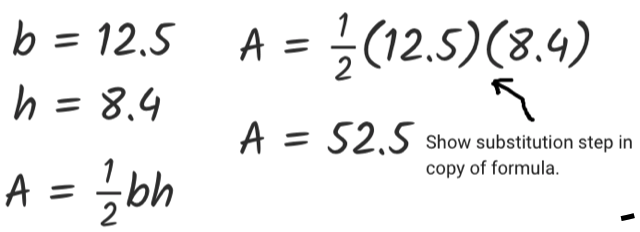
\includegraphics[width=8cm]{../graphics/04model-solution.png}
\end{flushright}

\item Find the area of a semi-circle with radius $r=7.5$. Paste a cropped screenshot of the Graspable Math. Compare your format to the model solution.
\item \vspace{4cm}
\begin{flushright}
  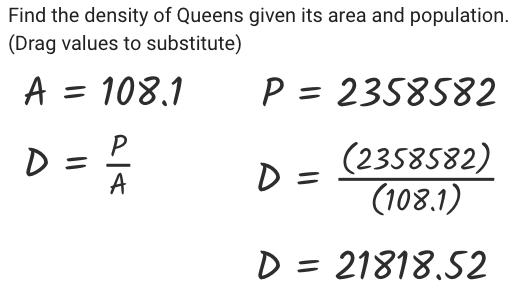
\includegraphics[width=10cm]{../graphics/04solution.png}
\end{flushright}

\item Find the population density of Queens, New York. Paste a cropped screenshot of the Graspable Math. Make a copy of the formula and show the substitution step.
\vspace{4cm}
\begin{flushright}
  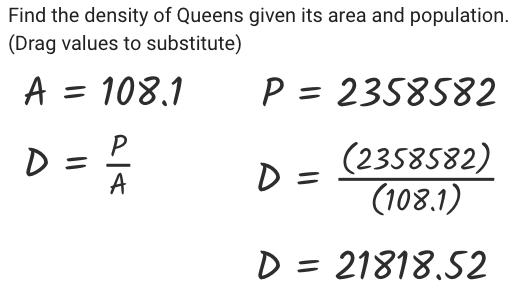
\includegraphics[width=9cm]{../graphics/04solution.png}
\end{flushright}


\end{enumerate}
\end{document}